\documentclass[english,14pt]{beamer}
\usetheme{EastLansing}
\usecolortheme{spruce}

\usepackage{xcolor}
\usepackage{listings}
\usepackage{courier}
\usepackage{graphicx}
\usepackage{amsmath}
\usepackage{algorithm2e}
\usepackage{multicol}
\usepackage{hyperref}
\usepackage{textcomp}

% http://mirrors.ibiblio.org/CTAN/macros/latex/contrib/datetime2/datetime2.pdf
\usepackage{babel}
\usepackage[useregional]{datetime2}

% https://tex.stackexchange.com/questions/42619/x-mark-to-match-checkmark
\usepackage{pifont}% http://ctan.org/pkg/pifont

%% https://stackoverflow.com/questions/1435837/how-to-remove-footers-of-latex-beamer-templates
%%gets rid of bottom navigation bars
%\setbeamertemplate{footline}[page number]
%
%gets rid of navigation symbols
\setbeamertemplate{navigation symbols}{}


\usefonttheme[onlymath]{serif}

\definecolor{mGreen}{rgb}{0,0.6,0}
\definecolor{mGray}{rgb}{0.5,0.5,0.5}
\definecolor{mPurple}{rgb}{0.8,0,0.82}
\definecolor{backgroundColour}{rgb}{0.95,0.95,0.92}
\definecolor{lightBlue}{rgb}{0.1, 0.1, 0.8}
\definecolor{darkGreen}{rgb}{0, 0.39, 0}

\newcommand\red[1]{{\color{red} #1}}
\newcommand\green[1]{{\color{green} #1}}
\newcommand\blue[1]{{\color{blue} #1}}
\newcommand\darkGreen[1]{{\color{darkGreen} #1}}

\newcommand{\cmark}{\ding{51}}%
\newcommand{\xmark}{\ding{55}}%

\lstdefinestyle{CStyle}{
    backgroundcolor=\color{backgroundColour},   
    commentstyle=\color{mGreen},
    keywordstyle=\color{magenta},
    numberstyle=\tiny\color{mGray},
    stringstyle=\color{mPurple},
    basicstyle=\footnotesize,
    breakatwhitespace=false,         
    breaklines=true,                 
    captionpos=b,                    
    keepspaces=true,                 
    numbers=left,                    
    numbersep=5pt,                  
    showspaces=false,                
    showstringspaces=false,
    showtabs=false,                  
    tabsize=2,
    language=Python
}

\lstdefinestyle{pseudo}{
        basicstyle=\ttfamily\footnotesize,
        keywordstyle=\color{lightBlue},
        morekeywords={BEGIN,END,IF,ELSE,ENDIF,ELSEIF,PRINT,WHILE,RETURN,ENDWHILE,DO,FOR,TO,IN,ENDFOR,BREAK,INPUT,CONDITIONS},
        morecomment=[l]{//},
        commentstyle=\color{mGreen}
}

\lstset{basicstyle=\footnotesize\ttfamily,breaklines=true}
\lstset{framextopmargin=50pt,tabsize=2}

\title{ENGG1003 - Thursday Week 10}
\subtitle{Assignment 2: Image processing}
\author{Steve Weller}
\institute{University of Newcastle}
%\date{\today}
\date{13 May 2021}

% following is a bit of a hack, but forces page numbers (technically: frame numbers) to run 1,2,3,... 
% with titlepage counting as frame 1

\addtocounter{framenumber}{1}
\titlepage

\begin{document}

\begin{flushleft}
{\scriptsize Last compiled:~\DTMnow}
\vspace*{-5mm}
\end{flushleft}
\framebreak

%==============================================================

\begin{frame}[fragile]

\frametitle{Lecture overview}
\begin{enumerate}
	\item key assignment information

	\item[]

	\item images as 3D arrays
	
	\item[]

	\item digital image formats

	\item[]

	\item data types

	\item[]

	\item structure of assignment

	\item[]

	\item strategies for the assignment

\end{enumerate}

\end{frame}

%==============================================================

\begin{frame}[fragile]

\frametitle{$1)$ Key assignment information}

\begin{itemize}
	\item released: Monday 10 May 2021
	\item \textbf{due date: 9:00am Monday 31 May 2021}
	\begin{itemize}
		\item Monday of week 13
	\end{itemize}
	\item weighting: 15\% of final course grade
	\item assignment sheet in BB $>$ assessment
	\begin{itemize}
		\item ensure you always have latest version
	\end{itemize}
	\item submission: upload \texttt{imageProcessing.py} file to BB as an assignment submission
	\item marking: during face-face labs in week 13
	\begin{itemize}
		\item final exam is on Tuesday of ``week 14'' (8 June)
	\end{itemize}
	\item marking guide released earlier today; details page 15 this lecture	
\end{itemize}

\end{frame}

%==============================================================

\begin{frame}[fragile]

\frametitle{$2)$ Images as 3D arrays}
\vspace*{-5mm}
\begin{figure}[ht]
	\centering
	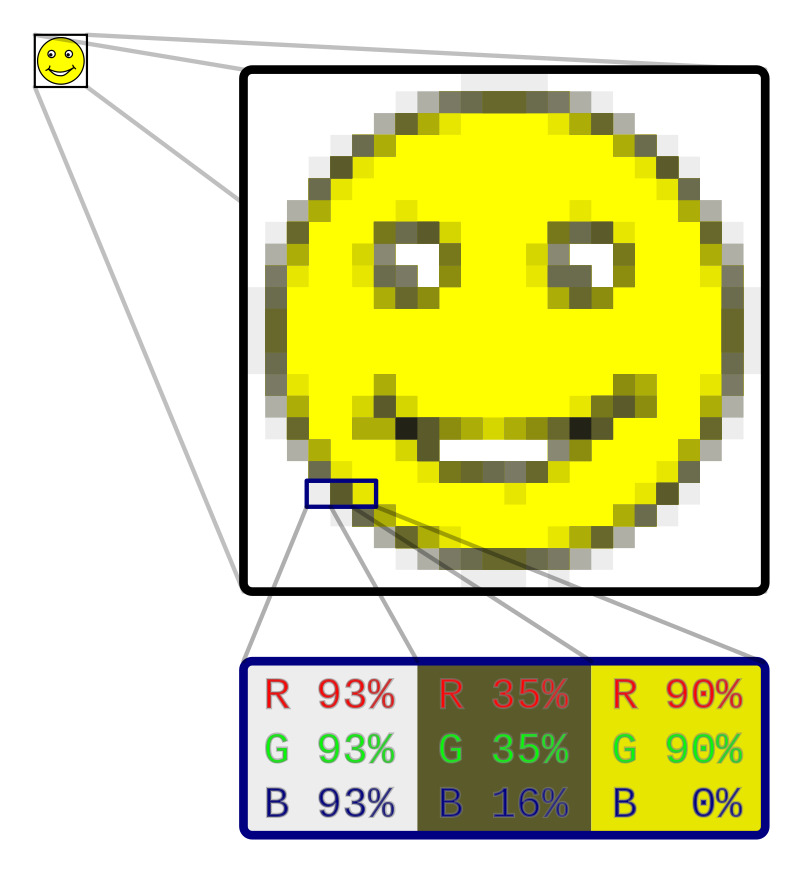
\includegraphics[width=.5\textwidth]{figures/smiley}
\end{figure}
\vspace*{-5mm}
{\footnotesize
\href{https://en.wikipedia.org/wiki/Raster_graphics}{https://en.wikipedia.org/wiki/Raster\_graphics} \\
\vspace*{-1mm}
CC0 1.0}

\end{frame}

%==============================================================

\begin{frame}[fragile]
\frametitle{Colour image as a 3D array}
\begin{itemize}
	\item think of 3D array as a 2D array where each entry is itself a length-3 array specifying the colour in RGB (red, green, blue) format
	\begin{itemize}
		\item each [R,G,B] entry maps to one pixel
	\end{itemize}
	\item[]
\[
	\left[ \begin{tabular}{ccccc}
        & [R, G, B] & $\cdots$ & [R, G, B] & \\
        & [R, G, B] & $\cdots$ & [R, G, B] & \\
        & [R, G, B] & $\cdots$  & [R, G, B] & \\
        \end{tabular} \right]
	\]
	\item[]
	\item[] \textbf{Examples:}
	\item[] red: [255, 0 ,0] \qquad green: [0, 255, 0]  \\ blue: [0, 0, 255] \qquad purple: [65, 0, 125]
\end{itemize}
\end{frame}

%==============================================================

\begin{frame}[fragile]

\frametitle{$3)$ Digital image formats}

\begin{itemize}

	\item colourspaces
	\begin{itemize}
		\item RGB: red--green--blue
		\item HSL: hue--saturation--luminance
	\end{itemize}
	\item[]
	\item RGB and HSL are two different ways of representing the \emph{same} colour
	\begin{itemize}
		\item key theme of assignment: RGB $\longleftrightarrow$ HSL
	\end{itemize}
	\item[]
	\item intensity values stored as numbers with min/max values:
	\begin{itemize}
		\item floats in range $[0,1]$
		\item integers in range $[0,255]$
	\end{itemize}
	\item {\small \href{https://www.w3schools.com/colors/colors_picker.asp}{https://www.w3schools.com/colors/colors\_picker.asp}}
\end{itemize}

\end{frame}

%==============================================================

\begin{frame}[fragile]

\frametitle{$4)$ Data types}

Assignment makes heavy use of numpy datatypes:
\vspace*{5mm}
\begin{itemize}
	\item \texttt{uint8}
	\begin{itemize}
		\item integer $0$ to $255$
	\end{itemize}
	\item \texttt{uint16}
	\begin{itemize}
		\item integer $0$ to $65535$
	\end{itemize}
	\item \texttt{float32}
	\begin{itemize}
		\item single-precision float (occupies $32$ bits)
	\end{itemize}
	\item \texttt{float64}
	\begin{itemize}
		\item double-precision float (occupies $64$ bits)
	\end{itemize}	
\end{itemize}

\end{frame}

%==============================================================

\begin{frame}[fragile]

\frametitle{$5)$ Structure of assignment}

\begin{itemize}
	\item covers the basics of digital image manipulation
	\item you will learn how everyday tools such as mobile phone camera apps perform several common image processing tasks
	\item first 5 functions
	\begin{itemize}
		\item ``unconstrained'' help from discord, demonstrators, fellow students is permitted
		\item[] (your assignment submission must be your own work)
		\item no marks for these questions; required for later q's
	\end{itemize}
	\item next 8 functions
	\begin{itemize}
		\item where the marks are
		\item \emph{\textbf{functions can be attempted in any order! }}
		\item implement all 8 functions, or fewer (for fewer marks)
	\end{itemize}
\end{itemize}

\end{frame}

%==============================================================

\begin{frame}[fragile]

\frametitle{Five ``getting started'' functions}

\begin{itemize}
	\item \textbf{\blue{\texttt{loadImage()}}}
	\begin{itemize}
		\item read image file into 3D numpy array
	\end{itemize}
		
	\item \textbf{\blue{\texttt{saveImage()}}}
	\begin{itemize}
		\item save 3D numpy array as image file
	\end{itemize}
			
	\item \textbf{\blue{\texttt{rgb2hsl()}}}
	\begin{itemize}
		\item convert image in RGB format to HSL format
	\end{itemize}
			
	\item \textbf{\blue{\texttt{hsl2rgb()}}}
	\begin{itemize}
		\item convert image in HSL format to RGB format
	\end{itemize}
			
	\item \textbf{\blue{\texttt{showImage()}}}
	\begin{itemize}
		\item display image in window
	\end{itemize}
\end{itemize}

\end{frame}

%==============================================================

\begin{frame}[fragile]

\frametitle{Eight functions in the assignment}

Eight (8) functions to be graded in assignment

\vspace*{5mm}

\begin{itemize}
	\item \textbf{\red{\texttt{brightness()}}}
	\begin{itemize}
		\item adjust image brightness
	\end{itemize}
		
	\item \textbf{\red{\texttt{contrast()}}}
	\begin{itemize}
		\item adjust image contrast
	\end{itemize}
			
	\item \textbf{\red{\texttt{saturation()}}}
	\begin{itemize}
		\item adjust image saturation
	\end{itemize}
			
	\item \textbf{\red{\texttt{toneMap()}}}
	\begin{itemize}
		\item adjust image by setting H and S channels of each pixel
	\end{itemize}
\end{itemize}

\end{frame}

%==============================================================

\begin{frame}[fragile]

\frametitle{}

Eight (8) functions to be graded in assignment (ctd.)

\vspace*{5mm}

\begin{itemize}
	\item \textbf{\red{\texttt{crop()}}}
	\begin{itemize}
		\item crop image
	\end{itemize}
		
	\item \textbf{\red{\texttt{histogram()}}}
	\begin{itemize}
		\item plot histogram of image
	\end{itemize}
			
	\item \textbf{\red{\texttt{saturated()}}}
	\begin{itemize}
		\item compute percentage of pixels which have at least one RGB channel value which has undergone clipping saturation
	\end{itemize}
			
	\item \textbf{\red{\texttt{unsharpMask()}}}
	\begin{itemize}
		\item sharpen image
	\end{itemize}
\end{itemize}

\end{frame}

%==============================================================

\begin{frame}[fragile]

\frametitle{$6)$ Strategies for the assignment}

\begin{itemize}
	\item lots of useful and relevant info in the assignment sheet
	\item[]
	\item \emph{strongly} recommend completion of week 10 lab sheet before starting assignment
	\item[]
	\item start small, take tiny steps
	\item[]
	\item test RGB/HSL conversion against colour picker
\end{itemize}

\end{frame}

%==============================================================

\begin{frame}[fragile]

\frametitle{Strategies}

\begin{itemize}
	\item submission to BB will be a single file \texttt{imageProcessing.py}
	\begin{itemize}
		\item your uploaded file will contain definitions and code for 5+8 functions
		\item implement $<$~8 assessable functions, for $<$~15 marks
	\end{itemize}
	\item[]
	
	\item \textbf{\emph{strongly}} encouraged to develop and test as follows:
	\begin{enumerate}
		\item each function's behaviour in its own script (test it)
		\item define code into function in same file (test it again)
		\item copy/paste working function into \texttt{imageProcessing.py} (and test it again!)
		\begin{itemize}
			\item test code will be made available to students
			\item you can check \emph{in advance} if your code works correctly!
	\end{itemize}
	\end{enumerate}
\end{itemize}

\end{frame}

%==============================================================

\begin{frame}[fragile]

\frametitle{Strategies for developing code}

Step 1: in \texttt{square.py}
\begin{lstlisting}[style=CStyle,basicstyle=\scriptsize]
# square

x = 3
print('{} squared = {:.4f}'.format(x,x**2))
\end{lstlisting}

\pause

Step 2: in \texttt{square\_fn.py}
\begin{lstlisting}[style=CStyle,basicstyle=\scriptsize]
# square_fn
def f(x):
    return x**2

x = 3
print('{} squared = {:.4f}'.format(x,f(x)))
\end{lstlisting}

\pause

Step 3: in \texttt{imageProcessing.py}
\begin{lstlisting}[style=CStyle,basicstyle=\scriptsize]
def f(x):
    return x**2
\end{lstlisting}

\end{frame}
%==============================================================

\begin{frame}[fragile]

\frametitle{Code testing and grading}

\vspace*{-3mm}

\begin{itemize}
	\item 15 marks total, for 15\% assignment
	\item 2 marks each for correct implementation of:
	\begin{itemize}
		\item brightness()
		\item contrast()
		\item saturation()
		\item toneMap()
		\item crop()
		\item saturated()
		\item histogram()
	\end{itemize}
	\item 1 mark for correct implementation of:
	\begin{itemize}
		\item unsharpMask()
	\end{itemize}
\end{itemize}

\textbf{\emph{Python test script published on BB which allows you to judge the correctness of your implementations with easy-to-debug data}}

\end{frame}

\end{document}